% Chapter Template

\chapter{Introduction} % Main chapter title

\label{Chapter1} % Change X to a consecutive number; for referencing this chapter elsewhere, use \ref{ChapterX}

%----------------------------------------------------------------------------------------
%	SECTION 1
%----------------------------------------------------------------------------------------

\section{Motivation}

The use of deep learning in medical imaging has been on the rise over the last few years. It has widely been used in various tasks across medical imaging such as image segmentation  (\cite{ronneberger2015u,guo2019deep,sinha2019multi,dolz2018hyperdense,hatt2018first}), image denoising (\cite{kadimesetty2018convolutional,li2020sacnn,chen2017low,yang2018low}), image analysis (\cite{litjens2017survey,amyar20193,cui2018artificial}). %\noteAB{Add more references}. 
Deep learning based algorithms produce faster results along with best possible quality in accordance with existing state of the art methods (\cite{leuschner2021quantitative}). Medical Image reconstruction too has benefited hugely with the advancement of deep learning (\cite{reader2020deep,zhang2020review}).
Medical Image reconstruction corresponds to the task of mapping raw projection data retrieved from the detector to image domain data. During the course of this thesis, the focus has been towards \ac{PET} and \ac{CT} image reconstruction. Both these modalities present a unique of set of challenges for image reconstruction. 
 
\ac{PET} imaging is a form of emission tomography wherein the image reconstruction task revolves around identifying the radio-tracer distribution emitted from the patient. A \ac{PET} image gives functional information about the organs in a patient making it invaluable for oncology. Some of the challenges in \ac{PET} image reconstruction are scatter, attenuation and difficulty in identifying the exact annihilation point of the electron-positron. Despite being the most sensitive emission tomography modality, the number of photons captured is low relative to the photons emitted contributing to further image degradation. These challenges result in very noisy images when reconstructed with analytical algorithms. These challenges are addressed by  Iterative/Model-based approaches which take into account detector geometry, noise statistics and approximate scatter and attenuation correction resulting in better image quality. 

\ac{CT} imaging on the other hand is an example of transmission tomography. The extent of attenuation undergone by X-Rays that pass through a patient are measured to obtain attenuation maps. In \ac{CT} imaging research, there has been active interest in sparse-view and low-dose reconstruction scenarios. In both cases, severe artifacts are introduced in  reconstructed images either due to incomplete projections or low counts. Many established model-based iterative methods account for the low-dose and sparse-view settings to remove artifacts and noise from the reconstruction (\cite{nuyts1998iterative,Elbakri2002,liu2013total}). However, these methods for require the knowledge of the noise and artifacts statistics and generally have longer reconstruction times (\cite{kim2014combining}). 


The main tasks involved in image reconstruction can be broadly categorized into three: sinogram correction, domain translation from sinogram to image, and image correction. Algorithms either tackle the three task individually or simultaneously account for them. One can relate to these tasks in the domain of Computer Vision wherein deep learning architectures have revolutionized the field by producing the state of the art results in most applications (\cite{guo2016deep}). For example, effective use of deep learning-based methods is seen in dealing with image denoising (\cite{kadimesetty2018convolutional,li2020sacnn,chen2017low,yang2018low}), super resolution (\cite{ledig2017photo,lim2017enhanced}) and image-to-image translation (\cite{isola2017image,zhu2017unpaired}) tasks. The continuous improvement in the availability of public data has further propelled interest in data-driven medical image reconstruction making it an active area of research. This thesis aims to explore novel deep learning approaches for \ac{PET} and \ac{CT} image reconstruction. Most common ways to introduce deep learning architectures in the image reconstruction pipeline are for pre-processing to correct raw projection data from the detector and post-processing to improve images reconstructed with existing methods. Another way is to embed the network into an iterative algorithm to enable faster convergence. The relatively less explored way called direct image reconstruction is to utilize neural networks alone for the entire reconstruction process. In this thesis \ac{CNN} approaches are proposed for direct image reconstruction with neural networks. 


\section{Thesis Organization}

This thesis is divided into six chapters with the first two chapters being introduction and literature review, followed by three chapters that focus on different deep learning methods explored during the thesis, and finally conclusion and perspectives. In the introduction various aspects of \ac{PET} and \ac{CT} image reconstruction are discussed along with the relevant background in deep learning background. The second chapter throws light on deep learning applied to medical image reconstruction and reviews the state of the art approaches in the scope of this thesis. 
In chapter 3 , we discuss reconstruction framework \ac{DUGAN} for \ac{PET} and \ac{CT} image reconstruction. A novel method for Sparse-view \ac{CT} reconstruction called \ac{LRRCED} is covered in chapter 4. A modified version of \ac{LRRCED} for total body \ac{PET} is discussed in chapter 5. Potential improvements and ideas for future work are presented in the final chapter. 

%----------------------------------------------------------------------------------------
%	SECTION 3
%----------------------------------------------------------------------------------------

\section{Imaging Modalities and Reconstruction Models}


%-----------------------------------
%	SUBSECTION 1
%-----------------------------------
\subsection{PET}


\ac{PET} images provide functional information to the radiologist making them invaluable in image analysis. The application of \ac{PET} imaging has been on the rise in oncology, cardiology and neuropsychiatry. The increased application lead to the development of many novel reconstruction approaches that lead to improved image quality. This section focuses on the standard analytical and iterative algorithms which are applicable in the context of this thesis. 

The aim of image reconstruction in \ac{PET} is to predict the tracer distribution emitted from the patient. The emission is a result of positron emitting radionuclide injected into the patient which causes positron-electron annihilation. The annihilation results in the production of gamma photons that travel in opposite directions due to the law of conservation of momentum. The simultaneous detection of these photons (also called coincidence events) enables the estimation of tracer distribution in \ac{PET} imaging. A \ac{PET} scanner detects the coincidence events through a set of detectors arranged in a circular fashion. This design of the scanner facilitates detection of coincidence photons between a pair of detectors ($d_p$ and $d_q$). The centers of two detectors are connected by a straight line called \ac{LOR}. Photon pairs that are not subject to scatter are a result of annihilation events that occur along a thin volume surrounding the \ac{LOR}. In \ac{PET}, $\boldx = \boldlambda$ is the distribution of a radiotracer delivered to the patient by injection, and is measured through the detection of pairs of $\gamma$-rays emitted in opposite directions (indirectly from the positron-emitting radiotracer).

\begin{figure}[!htbp]
	\centering
	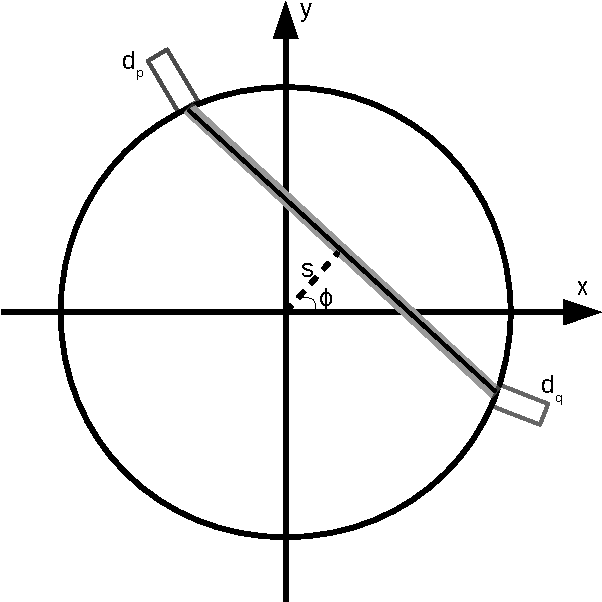
\includegraphics[width=0.6\linewidth]{./Figures/PET_det-crop.pdf}
	\caption{Depiction of a circular \ac{PET} detector with detectors $d_p$ and $d_q$ connected with a \ac{LOR} indicated in gray.}
	\label{fig:three}
\end{figure}


The measurement $\boldy$ is a random vector modeling the number of detection (photon counting) at each of the $n$ detector bins, and follows a Poisson distribution with independent entries:
\begin{equation}\label{eq:poisson}
\boldy \sim \mathrm{Poisson}(\boldybar(\boldx))
\end{equation}    
where $\boldybar(\boldx) \in \bbR^n$ is the expected number of counts (noiseless), which is a function of the image $\boldx$. 

The expected number of counts is
\begin{equation}\label{eq:PET}
\boldybar(\boldlambda) = \boldP \boldlambda
\end{equation}
where $\boldP \in \bbR^{n\times m}$ is a system matrix such that each entry $[\boldP]_{i,j}$ represents the probability that a photon pair emitted from voxel $j$. Image reconstruction is achieved by finding a suitable image $\boldxhat = \boldlambdahat$ that approximately solves 
\begin{equation}\label{eq:pb1solve}
\boldy = \boldybar(\boldx) \, .
\end{equation} 

%-----------------------------------
%	SUBSECTION 2
%-----------------------------------
\subsection{CT}
% Write a paragraph on CT imaging
Let an image be represented by $\boldx \in \bbR^m$ and the scanner measurement by $\boldb \in \bbR^n$ where $m$ is the number of voxels and $n$ is the number of measurements. In \ac{2D} \ac{CT} imaging $n$ depends on the number of detectors $N_\mathrm{d}$ and the number of angles $N_\mathrm{a}$. The task of medical image reconstruction corresponds to finding a mapping from $\boldb$ to $\boldx$. The measurement $\boldb$ is a random vector modeling the number of detection (photon counting) at each of the $n$ detector bins, and follows a Poisson distribution with independent entries, i.e.,
\begin{equation}\label{eq:pCT}
\boldb \sim \mathrm{Poisson}(\boldbbar(\boldx))
\end{equation}    
where, $\boldb  =  [b_1(\boldx),\dots,b_n(\boldx)]\transp\in \bbR^n$ and $\boldbbar(\boldx)  =  [\bbar_1(\boldx),\dots,\bbar_n(\boldx)]\transp\in \bbR^n$ is the expected number of counts (noiseless), which is a function of the image $\boldx$. 

The image $\boldx\in\mathbb{R}^m$ is a vectorized input image (also referred to as attenuation) representing the measure of X-rays absorbed or scattered as they pass through the patient. In a monochromatic setting, the expected number of counts $\boldbbar(\boldx)$  is given by the Beer-Lambert law, i.e.,
\begin{equation}\label{eq:CT}
\bbar_i(\boldx) = I \cdot \exp (-[\boldP \boldx]_i) \quad \forall i=1,\dots,n 
\end{equation}
where, $I$ is the intensity and $\boldP \in \bbR^{n\times m}$ is a system matrix such that each entry $[\boldP]_{i,j}$ represents the contribution of the $j$-th image voxel to the $i$-th detector. Given the raw projections $\boldbbar$, we take the logarithm as follows
\begin{equation}
y_i = \log\left(\frac{I}{b_i}\right) \quad \forall i=1,\dots,n   
\end{equation}
where we assumed that the intensity $I$ is sufficiently high so that $b_i>0$ for all $i$. Image reconstruction is based on finding a suitable image $\boldxhat$ that approximately solves 
\begin{equation}\label{eq:pb2solve}
\boldy = \boldP \boldxhat 
\end{equation} 
 
where $\boldy  =  [y_1,\dots,y_n]\transp\in \bbR^m$. The reconstruction can also be achieved with more sophisticated iterative techniques that account for the stochastic properties of the measurement \eqref{eq:poisson} \cite{nuyts1998iterative,Elbakri2002}.

In a sparse-view setting, the number of rotation angles of the detector is decreased in order to reduce the radiation passing through the patient. This implies a reduction in the number of projection angles in the measurement $\boldy$.


%-----------------------------------
%	SUBSECTION 3
%-----------------------------------
\subsection{Analytical Reconstruction Algorithms}
Analytical algorithms can efficiently solve \eqref{eq:pb1solve} and \eqref{eq:pb2solve} and have been the cornerstone of tomographic image reconstruction. One of the most famous reconstruction algorithms for both \ac{PET} and \ac{CT} is the \ac{FBP}. The projections ($\boldy$) are first filtered (typically with a ramp filter) and then back-projected to get an image. The discrete implementation of the \ac{FBP} can be written as follows:

\begin{equation}\label{eq:FBP}
	\boldx(i,j) = \frac{\pi}{N_\phi}\sum_{l=0}^{N_\phi-1}\boldy_f(s=i\cos\phi_l+j\sin\phi_l,\phi_l)
\end{equation}

where $x$ is the image for a set of pixels $(i,j)$, $\boldy_f$ are the filtered projections obtained by filtering the projections, expressed in terms of radial variable $s$ and projection angle $\phi$, and $N_\phi$ number of projection angles. The above equation is the approximation of backprojection by a discrete quadrature. 

Analytical methods are faster to implement and practical in a clinical setting but they are vulnerable to noise. The assumptions made in analytical formations are that the measurements are continuous and the solutions are of integral formulation. Sampling is done to the data a posteriori. They are also highly susceptible to system geometry. Since the 80's, \ac{MBIR} techniques \cite{Shepp1982,fessler2000statistical} became the standard approach. They consist in iteratively approximating a solution $\boldxhat$ such that $\boldybar(\boldxhat)$ maximizes the likelihood of the measurement $\boldy$. As they model the stochasticity of the system, they are more robust to noise as compared with \ac{FBP}, and can be completed with a penalty term for additional control over the noise \cite{depierro1995}. 
%-----------------------------------
%	SUBSECTION 4
%-----------------------------------
\subsection{Iterative Reconstruction Algorithms}

These algorithms are modeled on discrete representation of measurement and the image. They also incorporate corrections for scatter and are independent of detector geometry. Two different \ac{MBIR} methodologies, namely \ac{MLEM} and \ac{WLS} for \ac{PET} and \ac{CT} image reconstruction respectively, are discussed in this section. 
\subsubsection{\ac{MLEM}}
The key components of an iterative method are the data model, cost function and optimization. The cost function for \ac{MLEM} is based on Poisson likelihood given as follows:
\begin{equation}\label{eq:poisson_like}
\operatorname{Pr}\{\boldybar \mid \boldx\}=\prod_{j=1}^{N_{L o R}} \exp \left(-\left\langle y_{j}\right\rangle\right)\left\langle y_{j}\right\rangle^{y_{j}} / y_{j} !
\end{equation}

Putting \ref{eq:PET} in \ref{eq:poisson_like}, taking log and dropping terms that do not depend on unknown image $x$ we get the cost function for \ac{MLEM},

\begin{equation}
Q(\boldxbar, \boldybar)=\sum_{j=1}^{N_{L O R}}\left\{-\sum_{i=1}^{m} P_{j, i} x_{i}+y_{j} \log \left(\sum_{i=1}^{m} P_{j, i} x_{i}\right)\right\}
\end{equation}
where $Q$ is the cost function and the definition of other variables is consistent from above. As long as the matrix $P$ is singular, the above cost function remains convex and results in a unique image. 
The update step to map from the current estimate $x^{n}$ to the next estimate $x^{n+1}$ can be written as follows:

\begin{equation}
\boldxbar_{i}^{n+1}=x_{i}^{n} \frac{1}{\sum_{j^{\prime}=1}^{N_{L o R}} P_{j^{\prime}, i}} \sum_{j=1}^{N_{L O R}} P_{j, i} \frac{y_{j}}{\sum_{i^{\prime}=1}^{m} P_{j, i^{\prime}} x_{i^{\prime}}^{n}} \quad i=1, \ldots, m
\end{equation}

The initial estimate $x_i^{1}$, $i=1, \ldots, m$ typically follows a uniform distribution. The denominator with sum over index $i^{\prime}$ is the forward projection operation. Hence it estimates the measured data for the current image estimate. The numerator with sum over index $j$ is the back projection over the ratio of measured and estimated data. The \ac{MLEM} algorithm does not include a prior and it converges to the image that best fit the data. This estimate has inherent instabilities as the fitting is done closely to the noisy measured data. Various strategies like adding a Bayesian prior to the cost function, filtering the measured data or image post reconstruction, are employed to improve image quality. 

\subsubsection{\ac{WLS}}

One of the most common iterative techniques for \ac{CT} image reconstruction is the \ac{WLS} method, the image $\xhat$ is estimated by minimizing the following:

\begin{equation}
\hat{x}=\underset{x \succeq 0}{\arg \min } \frac{1}{2}\|y-A x\|_{W}^{2}
\end{equation}

where $W=\operatorname{diag}\left\{w_{i}\right\}$ is the diagonal weighting matrix that constitutes for the variance of each ray and $\|z\|_{W}^{2}=z^{\prime} W z$. Despite the statistical weighting, due to the noise in measurements and ill-conditioned problem of image reconstruction the image estimate will still be noisy. 

An improvement to the above can be brought by finding a balance between the desired a priori characteristics of the image and the data fitting. This balance is realized through a regularized \ac{WLS} cost function:

\begin{equation}
\hat{x}=\underset{x \succeq 0}{\arg \min } \Psi(x), \quad \Psi(x) \triangleq \frac{1}{2}\|y-A x\|_{W}^{2}+\beta R(x)
\end{equation} 


where $R(x)$ is the regularization term, that enforces piece-wise smoothness on the image and $\beta$ the regularization parameter. The usual choice for $R$ is an edge preserving regularizer that penalized the differences between neighboring voxels:

\begin{equation}
R(x)=\sum_{j=1}^{n_{\mathrm{p}}} \sum_{k \in \mathcal{N}_{j}} \psi_{j k}\left(x_{j}-x_{k}\right)
\end{equation}    

where $N_j$ are the set of neighboring indices of the $j^\mathrm{th}$ voxel. $\psi$ is a potential function that controls the penalization of differences in the neighboring voxels.

Sparse-view \ac{CT} image reconstruction problem has been explored during the course of this thesis. Sparse-view \ac{CT} image reconstruction is an under-determined problem due to the limited number of projection data available for reconstruction. In such a scenario stronger forms of regularization like \ac{TV} are utilized. Consider a 2D digital image $x[p,q]$, discrete form of \ac{TV} can be written as:

\begin{equation}
\sum_{p} \sum_{p}|x[p, q]-x[p-1, q]|+|x[p, q]-x[p, q-1]|
\end{equation}    

This is an an-isotropic version of \ac{TV} regularization. Images reconstructed with \ac{TV}, sometimes have inexplicable artifacts due to the fact that the absolute value potential is not differentiable at $0$. 

\section{Neural networks}

Neural networks also known as \ac{ANN} are machine learning algorithms that form the basis of deep learning. They inherit name and structure from neurons in the brain. Biological neurons transmit signals to one another through complex networks. This interconnected networking is realized though various architectures by \ac{ANN}s. Sets of artificial neurons are stacked on top of each other to form a layer. A typical neural network consists of many such layers that are connected to each other. The first layer is called input layer, the final layer is termed output layer and the layers in-between are called hidden layers. A neural network with three hidden layers is depicted in Fig~\ref{fig:nn}. The transmission of data across the nodes or artificial neurons happens through the connections. Each and every node has a specific weight and threshold associated. The output from a node is passed through the connection only if the value is above the threshold. Neural network approaches are data-driven. Their performance improves as they learn through training on a dataset. 

\begin{figure}
	\centering
\begin{neuralnetwork}[height=5]
	\newcommand{\x}[2]{$x_#2$}
	\newcommand{\y}[2]{$\hat{y}_#2$}
	\newcommand{\hfirst}[2]{\small $h^{(1)}_#2$}
	\newcommand{\hsecond}[2]{\small $h^{(2)}_#2$}
	\inputlayer[count=4, bias=true, title=Input\\layer, text=\x]
	\hiddenlayer[count=5, bias=false, title=Hidden\\layer 1, text=\hfirst] \linklayers
	\hiddenlayer[count=4, bias=false, title=Hidden\\layer 2, text=\hsecond] \linklayers
	\hiddenlayer[count=3, bias=false, title=Hidden\\layer 3, text=\hsecond] \linklayers
	\outputlayer[count=2, title=Output\\layer, text=\y] \linklayers
\end{neuralnetwork}
\caption{Depiction of a neural network with an input layer, three hidden layers and an output layer}\label{fig:nn}
\end{figure}


To further understand the working of a neural network, we can imagine each node to be solving the problem of linear regression. For example consider a node with four inputs ($x_i, i=1,2,\dots4$), four weights ($w_i, i=1,2,\dots4$) and a bias:

\begin{equation}
\sum_{i=1}^{m} w_{i} x_{i}+\text { bias }=w_{1} x_{1}+w_{2} x_{2}+w_{3} x_{3}+w_{4} x_{4}+\text { bias }
\end{equation}

The output of the node is the above summation after going through an activation function $f$:

\begin{equation}
\text { output }=f(x)=\left\{\begin{array}{l}
1 \text { if } \sum w_{1} x_{1}+b \geq 0 \\
0 \text { if } \sum w_{1} x_{1}+b<0
\end{array}\right.
\end{equation}

In the above example, the given activation function of this node propagates the value $1$ only when the weighted sum of it's inputs is non-negative. When the condition of an activation function are met the output of this node becomes an input to the node to which it's connected. Due to the process of forwarding values through a network, an \ac{ANN} is also called feed-forward network. Complex networks with multiple layers of these nodes are used in practical tasks. An important category of machine learning task is supervised learning. It involves training a neural network on labeled datasets. The goal of training a neural network is to minimize a cost function that enforces the closeness of predicted and real output labels. During the training the network reorganizes it's weights based on the loss function. This process of updating weights is called optimization. Each update is aimed at reaching a minimum of the loss function. A popular optimization method is gradient descent. It guides the model in the direction of reducing errors to reach an optima. The development of back-propagation \cite{rumelhart1986learning} has been instrumental in successful implementation of optimization algorithms for neural networks.  



